\documentclass[11pt]{beamer}
\usetheme{CambridgeUS}
\usepackage[utf8]{inputenc}
\usepackage{amsmath}
\usepackage{amsfonts}
\usepackage{amssymb}
\usepackage[
backend=biber,
style=alphabetic,
citestyle=authoryear
]{biblatex}

\newcommand\Fontvi{\fontsize{8}{7.2}\selectfont}

% Footnote without number
\newcommand\blfootnote[1]{%
  \begingroup
  \renewcommand\thefootnote{}\footnote{#1}%
  \addtocounter{footnote}{-1}%
  \endgroup
}
\newcommand{\comment}[1]{}

\addbibresource{stats.bib}
\title[Bioestatística II] %optional
{Introdução à Bioestatística}

\subtitle{CGF2046 - Bioestatística II}

\author[da Silva, Ricardo] % (optional, for multiple authors)
{R. ~R. ~da Silva\inst{1}}

\institute[FCFRP] % (optional)
{
  \inst{1}%
  Departamento de Ciências BioMoleculares\\
  Faculdade de Ciências Farmacêuticas

}

\date{\today} % (optional)

\titlegraphic{\includegraphics[width=5.8cm]{figs/logo_final}} 

\begin{document}

\begin{frame}
\titlepage
\end{frame}

\begin{frame}
\label{contents}
\frametitle{Sumário}
\tableofcontents
\end{frame}


\section{Introdução}
\setbeamercovered{transparent}
\begin{frame}
\frametitle{Tipos de fenômenos}
%\Fontvi

  \uncover<1->{

\begin{block}{Fenômenos determinísticos}
Dizemos que um experimento é determinístico quando repetido inúmeras
vezes, \textbf{em condições semelhantes}, conduz a resultados
\emph{essencialmente} idênticos. Ex.:

\begin{itemize}
\Fontvi
\item
  Aceleração da gravidade;
\item
  Leis da Física e da Química.
\end{itemize}

\end{block}
  }

  \uncover<2->{

\begin{block}{Fenômenos aleatórios}

Os experimentos que \textbf{repetidos sob as mesmas condições} geram
resultados diferentes, são chamados de experimentos aleatórios. Ex.:

\begin{itemize}
\Fontvi
\item
  Lançamento de uma moeda;
\item
  Lançamento de um dado;
\item
  Condições climáticas do próximo domingo;
\item
  Taxa de inflação do próximo mês.
\end{itemize}
\end{block}
  }

\end{frame}

\setbeamercovered{transparent}
\begin{frame}
\frametitle{Teoria das Probabilidades}

  \uncover<1->{
  O que é a Teoria das Probabilidades?

  \begin{itemize}
  \item
    Ramo da matemática que desenvolve e avalia \textbf{modelos} para
    descrever \textbf{fenômenos aleatórios}.
  \item
    É a base teórica para o desenvolvimento das técnicas estatísticas.
  \end{itemize}
  }

  \uncover<2->{
    Qual o objetivo da Teoria das Probabilidades?
    \begin{itemize}
    \item Construir um arcabouço matemático adequado para descrever
    \textbf{fenômenos aleatórios}.
    \end{itemize}
  }  
  \uncover<3->{
  O que precisamos para começar?

  \begin{itemize}
  \item
    Descrever o \textbf{conjunto} de resultados possíveis do
    \textbf{fenômeno aleatório} de interesse;
  \item
    Atribuir \textbf{pesos} a cada possível resultado, refletindo suas
    chances de ocorrência.
  \end{itemize}
  }
\end{frame}

\setbeamercovered{transparent}
\begin{frame}
\frametitle{Elementos da Teoria dos Conjuntos}

  \uncover<1->{
  \textbf{Espaço amostral}: Conjunto de todos os possíveis resultados de
  um experimento aleatório.
  \begin{itemize}
  \item
    Pode conter um número finito ou infinito de pontos.
  \item
    Exemplos: \{cara, coroa\}, \{1,2,3,4,5,6\}, \(\mathbb{R}^+\).
  \item
    Notação \(\Omega\).
  \end{itemize}
  }
  \uncover<2->{
  \textbf{Pontos amostrais}: São os elementos que compõem o \(\Omega\).

  \begin{itemize}
  \item
    Notação \(\omega\).
  \item
    Exemplo: \(\omega_1 = \text{cara}\), \(\omega_2 = \text{coroa}\).
  \end{itemize}
  }
  \uncover<3->{
  \textbf{Eventos}: Todo resultado ou \underline{subconjunto} de
  resultados de um experimento aleatório.

  \begin{itemize}
  \item
    Exemplos: A = ``sair cara'', B = ``sair face par''.
  \item
    Em geral são denotados por \(A, B, C \ldots\).
  \end{itemize}
  }
  
\end{frame}

\setbeamercovered{transparent}
\begin{frame}
\frametitle{Exemplos}

  \uncover<1->{
  \begin{examples}
  \begin{itemize}
\item
  \textbf{Experimento:} retirar uma carta de um baralho de 52 cartas.
\item
  \textbf{Espaço amostral:}
  \(\Omega=\{\clubsuit A,\clubsuit 2,...,\heartsuit A,...,\spadesuit A, ...,\diamondsuit J, \diamondsuit Q, \diamondsuit K\}\).
\item
  \textbf{Pontos amostrais:} \(\omega_1=\clubsuit A\),
  \(\omega_2=\clubsuit 2\), \ldots{}, \(\omega_{52}=\diamondsuit K\).
\item
  \textbf{Eventos:} A = ``sair um ás'', B = ``sair uma letra'', C =
  ``sair carta de \(\clubsuit\)''.
\end{itemize}
  \end{examples}
  }

  \uncover<2->{
  \begin{examples}
\begin{itemize}
\item
  \textbf{Experimento:} pesar um fruto ao acaso.
\item
  \textbf{Espaço amostral:} \(\Omega=\mathbb{R}^{+}\).
\item
  \textbf{Pontos amostrais:} espaço amostral é infinito.
\item
  \textbf{Eventos:} A = ``peso menor que 50g'', B =
  \(\{x: x\geq100\text{g}\}\).
\end{itemize}
  \end{examples}
  }
\end{frame}

\setbeamercovered{transparent}
\begin{frame}
\frametitle{Operações com eventos}

Usamos a \textbf{Teoria dos conjuntos} para definir operações com
eventos.

\begin{itemize}
  \uncover<1->{\item
  \textbf{Conjunto vazio} é o conjunto sem elementos, denotado por
  \(\emptyset\).
  }
  \uncover<2->{\item
  \textbf{União} é o evento que consiste da união de \textbf{todos} os
  pontos amostrais dos eventos que a compõem. Denotamos a união do
  evento A com B por \(A\cup B\).
  \(A \cup B = \{\omega \in A \text{ ou } \omega \in B\}\).
  }
  \uncover<3->{\item
  \textbf{Interseção} é o evento composto pelos pontos amostrais
  \textbf{comuns} aos eventos que a compõem. Denotamos a interseção de A
  com B por \(A \cap B\).
  \(A \cap B = \{\omega \in A \text{ e } \omega \in B\}\).
  }
\end{itemize}
\end{frame}

\setbeamercovered{transparent}
\begin{frame}
\frametitle{Operações com eventos}

Usamos a \textbf{Teoria dos conjuntos} para definir operações com
eventos.

\begin{itemize}
  \item
  \textbf{Conjunto vazio} é o conjunto sem elementos, denotado por
  \(\emptyset\).
  \item
  \textbf{União} é o evento que consiste da união de \textbf{todos} os
  pontos amostrais dos eventos que a compõem. Denotamos a união do
  evento A com B por \(A\cup B\).
  \(A \cup B = \{\omega \in A \text{ ou } \omega \in B\}\).
  \textbf{Interseção} é o evento composto pelos pontos amostrais
  \textbf{comuns} aos eventos que a compõem. Denotamos a interseção de A
  com B por \(A \cap B\).
  \(A \cap B = \{\omega \in A \text{ e } \omega \in B\}\).
\end{itemize}

\begin{center}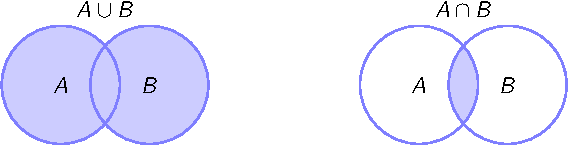
\includegraphics[width=0.9\linewidth]{figs/regra_adicao1-crop} \end{center}

\end{frame}

\begin{frame}
\frametitle{Tipos de eventos}
  \textbf{Disjuntos} (mutuamente exclusivos) são eventos que possuem
  interseção nula, ou seja, \(A\cap B = \{\emptyset\}\). \scriptsize

\begin{center}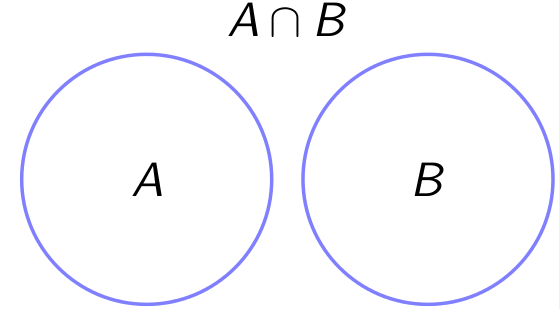
\includegraphics[width=0.25\linewidth]{figs/Disjuntos} \end{center}

\end{frame}

\begin{frame}
\frametitle{Tipos de eventos}

  \textbf{Disjuntos} (mutuamente exclusivos) são eventos que possuem
  interseção nula, ou seja, \(A\cap B = \{\emptyset\}\). \scriptsize

\begin{center}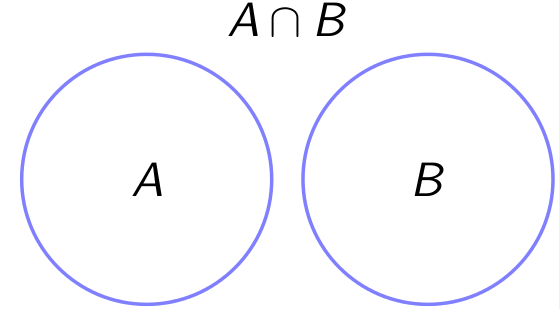
\includegraphics[width=0.25\linewidth]{figs/Disjuntos} \end{center}

  \textbf{Complementares} são eventos que a união é o espaço amostral,
  ou seja, \(A\cup A^{c} = \Omega\). \scriptsize

\begin{center}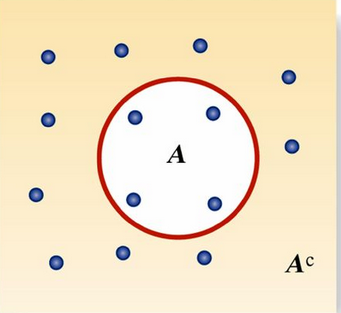
\includegraphics[width=0.25\linewidth]{figs/Comp} \end{center}
\end{frame}

\begin{frame}
\frametitle{Exemplo}

Considere o lançamento de um dado e os eventos: \(A = \{1,2,3,4\}\),
\(B = \{\omega:\omega\leq 3\}\), \(C = \text{face par}\),
\(D = \text{face
primo}\).

\begin{itemize}
\item
  Uniões

  \begin{itemize}
  \item
    \(A\cup B =\)
  \item
    \(A\cup C =\)
  \item
    \(A\cup D =\)
  \end{itemize}
\item
  Interseções

  \begin{itemize}
  \item
    \(A\cap B =\)
  \item
    \(A\cap C =\)
  \item
    \(A\cap D =\)
  \end{itemize}
\item
  Complementos

  \begin{itemize}
  \item
    \(A^c =\)
  \item
    \(B^c =\)
  \item
    \(D^c =\)
  \end{itemize}
\end{itemize}
\end{frame}

\begin{frame}
\frametitle{Exemplo}

Considere o lançamento de um dado e os eventos: \(A = \{1,2,3,4\}\),
\(B = \{\omega:\omega\leq 3\}\), \(C = \text{face par}\),
\(D = \text{face
primo}\).

\begin{itemize}
\item
  Uniões

  \begin{itemize}
  \item
    \(A\cup B = \{1,2,3,4\} \text{ou} \{1,2,3\} = \{1,2,3,4\}\)
  \item
    \(A\cup C = \{1,2,3,4\} \text{ou} \{2,4,6\} = \{1,2,3,4,6\}\)
  \item
    \(A\cup D = \{1,2,3,4\} \text{ou} \{2,3,5\} = \{1,2,3,4,5\}\)
  \end{itemize}
\item
  Interseções

  \begin{itemize}
  \item
    \(A\cap B = \{1,2,3,4\} \text{ou} \{1,2,3\} = \{1,2,3\}\)
  \item
    \(A\cap C = \{1,2,3,4\} \text{ou} \{2,4,6\} = \{2,4\}\)
  \item
    \(A\cap D = \{1,2,3,4\} \text{ou} \{2,3,5\} = \{2,3\}\)
  \end{itemize}
\item
  Complementos

  \begin{itemize}
  \item
    \(A^c = \{5,6\}\)
  \item
    \(B^c = \{\omega: \omega> 3\}\)
  \item
    \(D^c = \{1,4,6\}\)
  \end{itemize}
\end{itemize}
\end{frame}

\section{Probabilidade}
\setbeamercovered{transparent}
\begin{frame}
\frametitle{Definição axiomática de probabilidade}

Probabilidade é uma função \(P(\cdot)\) que atribui valores numéricos
aos eventos do espaço amostral, de tal forma que \\~\\

\begin{enumerate}
\def\labelenumi{\roman{enumi}.}

\uncover<1->{\item
  \(0 \leq P(A) \leq 1, \quad \forall A \in \Omega\); \\~\\
  }
\uncover<2->{\item
  \(P(\Omega) = 1\);\\~\\
  }
\uncover<3->{\item
  \(P(\bigcup_{j=1}^n A_j) = \sum_{j=1}^n P(A_j)\), com os \(A_j\)'s
  disjuntos. \\~\\
  }
\end{enumerate}

\uncover<4->{
A pergunta que surge é então: como atribuir probabilidades aos elementos
do espaço amostral?
}
\end{frame}

\setbeamercovered{transparent}
\begin{frame}
\frametitle{Definição de probabilidade}

Existem duas maneiras principais de atribuir probabilidades aos
elementos do espaço amostral:

\begin{enumerate}
\def\labelenumi{\arabic{enumi}.}
\item
  (\textbf{Clássica}) baseia-se nas características teóricas da
  realização do fenômeno.

  \begin{itemize}
  \item
    Considerando o lançamento de um dado, temos
    \(\Omega=\{1,2,3,4,5,6\}\)
  \item
    Admitindo que o dado é honesto, podemos assumir que
    \(P(1) = P(2) = \cdots = P(6) = 1/6\)
  \end{itemize}
\item
  (\textbf{Frequentista}) baseia-se nas frequências (relativas) de
  ocorrência do fenômeno.

  \begin{itemize}
  \item
    Determinar a probabilidade de ocorrência de cada face de um dado.
  \item
    Sem fazer nenhuma suposição inicial, podemos usar as
    \textbf{frequências relativas} de sucessivas ocorrências.
  \end{itemize}
\end{enumerate}
\end{frame}

\setbeamercovered{transparent}
\begin{frame}
\frametitle{Definição frequentista}

Podemos então pensar em repetir o experimento aleatório \(n\) vezes, e
contar quantas vezes o evento \(A\) ocorre, \(n(A)\).

Dessa forma a frequência relativa de \(A\) nas \(n\) repetições será

\[
f_{A,n} = \frac{n(A)}{n}.
\]

Para \(n \rightarrow \infty\) repetições sucessivas e independentes, a
frequência relativa de \(A\) tende para uma constante \(P(A)\), ou seja,

\[
\lim_{n \rightarrow \infty} \frac{n(A)}{n} = P(A).
\]

\textbf{Exemplo:} Se um dado fosse lançado \(n\) vezes, e contássemos
quantas vezes saiu a face 4, qual seria a probabilidade desse evento?
\end{frame}

\setbeamercovered{transparent}
\begin{frame}
\frametitle{Definição frequentista}

\begin{center}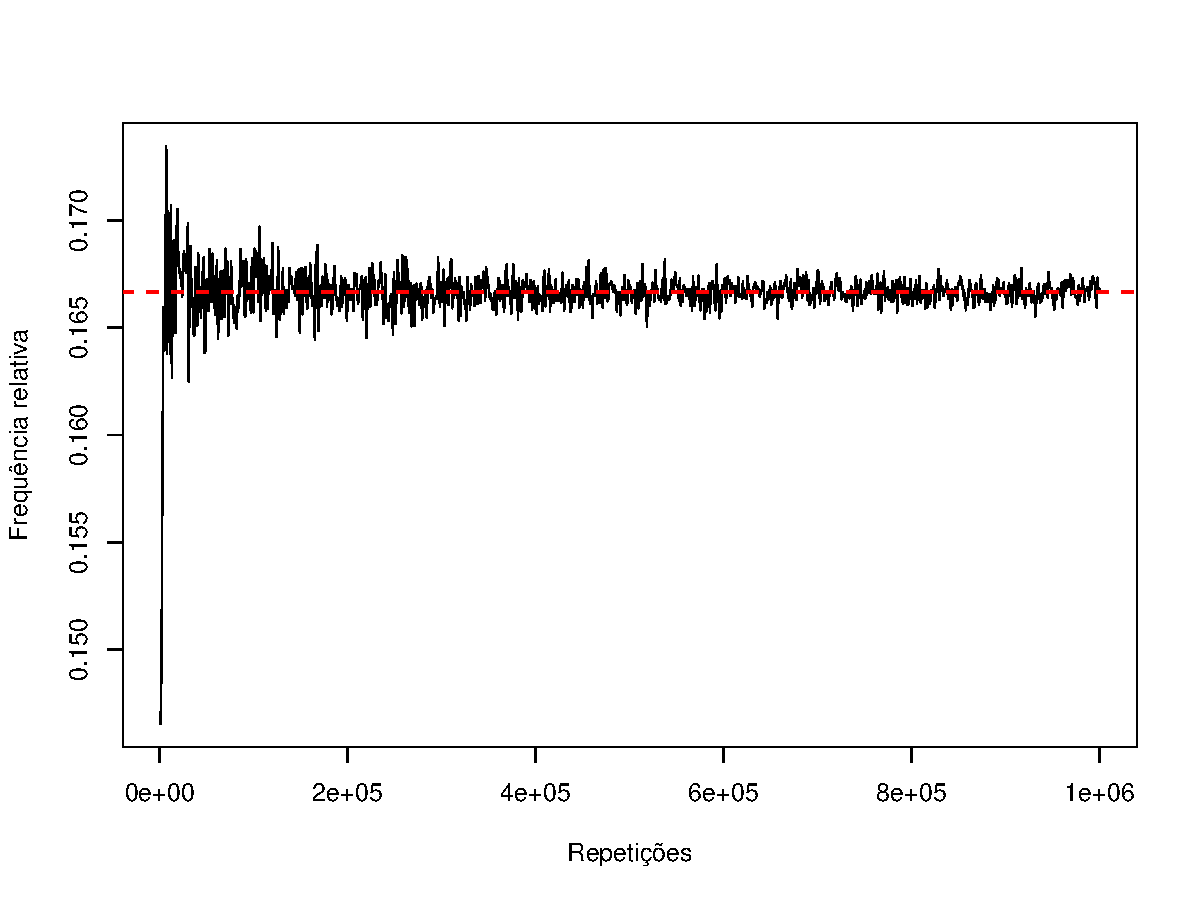
\includegraphics[width=0.8\linewidth]{figs/prob_freq} \end{center}
\end{frame}

\setbeamercovered{transparent}
\begin{frame}
\frametitle{Definição frequentista}

Assim,

\[
\lim_{n \rightarrow \infty} \frac{n(A)}{n} = P(A) \approx 0,1667.
\]

As probabilidades calculadas baseadas em frequências relativas, são
\textbf{estimativas} da verdadeira probabilidade.

À medida que o número de repetições vai aumentando, as
\textbf{frequências relativas} se estabilizam em um número que chamamos
de \textbf{probabilidade}.

\begin{alertblock}{Lei dos Grandes Números}

A Lei dos Grandes Números nos diz que as estimativas dadas pelas
frequências relativas tendem a ficar melhores com mais observações.
\end{alertblock}
\end{frame}


\setbeamercovered{transparent}
\begin{frame}
\frametitle{Exemplo}
\Fontvi
Considerando os dados da variável \texttt{Idade} da aula anterior e
considerando que os nossos dados são \textbf{populacionais}, tem-se

\begin{itemize}
\item
  O espaço amostral é \(\Omega = \{17, 18, \ldots, 25\}\).
\item
  Se um aluno é escolhido ao acaso, definimos a probabilidade dele ter
  certa idade pela frequência relativa
\end{itemize}

\begin{columns}
\column{.5\textwidth}

\begin{table}[ht]
\centering
\begin{tabular}{rrrr}
  \hline
 & $n_i$ & $f_i$ & $f_{ac}$ \\ 
  \hline
17 & 9 & 0.18 & 0.18 \\ 
  18 & 22 & 0.44 & 0.62 \\ 
  19 & 7 & 0.14 & 0.76 \\ 
  20 & 4 & 0.08 & 0.84 \\ 
  21 & 3 & 0.06 & 0.90 \\ 
  22 & 0 & 0.00 & 0.90 \\ 
  23 & 2 & 0.04 & 0.94 \\ 
  24 & 1 & 0.02 & 0.96 \\ 
  25 & 2 & 0.04 & 1.00 \\ 
   \hline
Sum & 50 & 1.00 &  \\ 
   \hline
\end{tabular}
\end{table}

\normalsize \column{.5\textwidth} \[
P(17) = 0,18; \ldots; P(25) = 0,04
\]
\end{columns}
\end{frame}

\setbeamercovered{transparent}
\begin{frame}
\frametitle{Exemplo}

Considerando os dados das variáveis \texttt{Sexo} e \texttt{Turma}


\begin{table}[ht]
\centering
\begin{tabular}{rrrr}
  \hline
 & F & M & Sum \\ 
  \hline
A & 21 & 5 & 26 \\ 
  B & 16 & 8 & 24 \\ 
   \hline
Sum & 37 & 13 & 50 \\ 
   \hline
\end{tabular}
\end{table}


Podemos extrair as seguintes probabilidades

\begin{align*}
P(F) = \frac{37}{50} = 0,74; P(M) = \frac{13}{50} = 0,26 \\
P(A) = \frac{26}{50} = 0,52; P(B) = \frac{24}{50} = 0,48.
\end{align*}

Qual seria a probabilidade de escolhermos ao acaso um estudante do sexo
feminino ou alguém da Turma B?
\end{frame}

\setbeamercovered{transparent}
\begin{frame}
\frametitle{Exemplo}

Queremos então \(P(F \cup B)\)

\begin{align*}
P(F \cup B) &= P(F) + P(B) \\
&= 0,74 + 0,48 \\
&= 1,22
\end{align*}

o que não é possível pois a soma é superior a 1.

Não é difícil ver que estamos somando alguns indivíduos 2 vezes, pois os
estudantes do sexo feminino e da turma B, ou seja, o evento \(F \cap B\)
está incluído no evento \(F\) e no evento \(B\).
\end{frame}

\setbeamercovered{transparent}
\begin{frame}
\frametitle{Exemplo}

Logo, precisamos subtrair \(P(F \cap B)\) para obter a probabilidade
correta.

Neste caso, pela tabela, vemos que a interseção \(F \cap B\) resulta na
probabilidade

\begin{align*}
P(F \cap B) = \frac{16}{50} = 0,32.
\end{align*}

E o resultado correto para \(P(F \cup B)\) é

\begin{align*}
P(F \cup B) &= P(F) + P(B) - P(F \cap B) \\
&= 0,74 + 0,48 - 0,32 \\
&= 0,9.
\end{align*}
\end{frame}


\setbeamercovered{transparent}
\begin{frame}
\frametitle{Regra da adição de probabilidades}

A probabilidade da união entre dois eventos quaisquer, \(A\) e \(B\), é
dada pela \textbf{regra da adição de probabilidades}

\[
P(A \cup B) = P(A) + P(B) - P(A \cap B).
\]

\begin{center}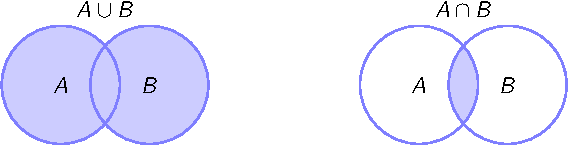
\includegraphics[width=0.7\linewidth]{figs/regra_adicao1-crop} \end{center}
\end{frame}

\setbeamercovered{transparent}
\begin{frame}
\frametitle{Regra da adição de probabilidades}

Note que a regra da adição pode ser simplificada, \textbf{se e somente
se} os eventos \(A\) e \(B\) forem \textbf{disjuntos} (ou mutuamente
exclusivos)

\[
P(A \cup B) = P(A) + P(B),
\]

pois, neste caso,
\(A \cap B = \emptyset \quad \Rightarrow \quad P(A \cap B) = P(\emptyset) = 0\).

\begin{center}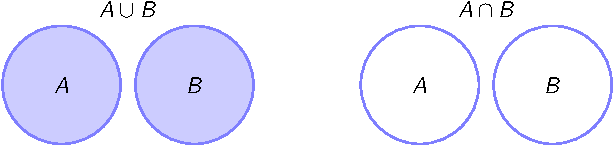
\includegraphics[width=0.7\linewidth]{figs/regra_adicao2-crop} \end{center}

\end{frame}

\setbeamercovered{transparent}
\begin{frame}
\frametitle{Regra do complementar}

Como consequência da regra da adição, temos que, para qualquer evento
\(A\),

\[
P(A) = 1 - P(A^c).
\]

Verifique através de \(P(A \cup A^c) = P(A) + P(A^c) - P(A \cap A^c)\).

\begin{eqnarray*} 
P(A \cup A^c) &=& 1. \quad \text{Pela regra da adição, tem-se} \\
P(A) + P(A^c) - P(A \cap A^c) &=& 1. \quad \text{interseção é nula, então} \\
P(A) + P(A^c) &=& 1. \quad \text{e portanto} \\
P(A) &=& 1 - P(A^c).
\end{eqnarray*}

\end{frame}

\section{Probabilidade condicional e independência}
\setbeamercovered{transparent}
\begin{frame}
\frametitle{Probabilidade condicional}

Em muitas situações práticas, o fenômeno aleatório com o qual
trabalhamos pode ser separado em etapas.

A informação do que ocorreu em uma determinada etapa pode influenciar
nas probabilidades de ocorrências das etapas sucessivas.

Nestes casos, dizemos que \textbf{ganhamos informação}, e podemos
\emph{recalcular} as probabilidades de interesse.

Estas probabilidades \emph{recalculadas} recebem o nome de
\textbf{probabilidades condicionais}.
\end{frame}

\setbeamercovered{transparent}
\begin{frame}
\frametitle{Definição}

\begin{itemize}
\item
  Dados dois eventos A e B, a probabilidade condicional de A ocorrer,
  dado que ocorreu B é representado por \(P(A | B)\) e dada por \[
  P(A | B) = \frac{P(A \cap B)}{P(B)}, \quad \text{para} \quad P(B) > 0.
  \]
\item
  Caso \(P(B) = 0\), definimos \(P(A | B) = P(A).\)
\end{itemize}
\end{frame}

\setbeamercovered{transparent}
\begin{frame}
\frametitle{Probabilidade condicional}

Considere o seguinte exemplo:

\begin{itemize}
\item
  Um dado foi lançado, qual é a probabilidade de ter ocorrido face 4?
\item
  Suponha que o dado foi jogado, e, sem saber o resultado, você recebe a
  informação de que ocorreu face par. Qual é a probabilidade de ter
  saido face 4 com essa ``nova'' informação?
\end{itemize}

\(\Omega = \{1,2,3,4,5,6\}\), \(n(\Omega) = 6.\)

\(A\) = face 4 = \(\{4\}\),
\(n(A) = 1 \quad \Rightarrow \quad P(A) = \frac{n(A)}{n(\Omega)} = \frac{1}{6}.\)

\(B\) = face par = \(\{2,4,6\}\),
\(n(B) = 3 \quad \Rightarrow \quad P(B) = \frac{n(B)}{n(\Omega)} = \frac{3}{6}.\)

\(C\) = face 4, dado que ocorreu face par = \(\{4\}\),
\(n(C) = \frac{1}{3}.\)

\end{frame}

\setbeamercovered{transparent}
\begin{frame}
\frametitle{Probabilidade condicional}

Usando a definição formal:

\(P(A \cap B) = \frac{n(A \cap B)}{n(\Omega)} = \frac{1}{6}\)

\(P(B) = \frac{n(B)}{n(\Omega)} = \frac{3}{6}\)

\begin{align*}
P(A|B) &= \frac{P(A \cap B)}{P(B)} \\
&= \frac{1/6}{3/6} \\
&= \frac{1}{3}.
\end{align*}
\end{frame}

\setbeamercovered{transparent}
\begin{frame}
\frametitle{Regra do produto}

A regra do produto é uma expressão derivada do conceito de probabilidade
condicional. Uma vez que

\[
P(A|B) = \frac{P(A\cap B)}{P(B)}
\]

temos que

\[
P(A\cap B) = P(A|B) \cdot P(B)  .
\]

Essa expressão permite calcular probabilidades em espaços amostrais que
são realizados em sequência, onde a ocorrência da \emph{segunda} etapa
\textbf{depende} (ou não) da ocorrência da \emph{primeira} etapa.
\end{frame}

\setbeamercovered{transparent}
\begin{frame}
\frametitle{Regra do produto}

Qual a probabilidade de se obter dois ases em seguida, quando se extraem
duas cartas de um baralho comum de 52 cartas, se:

\begin{enumerate}
\def\labelenumi{\alph{enumi}.}
\item
  A primeira carta extraída \textbf{não} é reposta antes da extração da
  segunda carta.
\item
  A primeira carta é reposta no baralho antes da extração da segunda
  carta.
\end{enumerate}
\end{frame}

\setbeamercovered{transparent}
\begin{frame}
\frametitle{Eventos independentes}

Vimos que para probabilidades condicionais, \(P(A|B)\), saber que \(B\)
ocorreu nos dá uma informação ``extra'' sobre a ocorrência de \(A\).

Porém, existem algumas situações nas quais saber que o evento \(B\)
ocorreu, não tem qualquer interferência na ocorrência ou não de \(A\).

Nestes casos, podemos dizer que os eventos \(A\) e \(B\) são
\textbf{independentes}.
\end{frame}

\setbeamercovered{transparent}
\begin{frame}
\frametitle{Eventos independentes}

Os eventos A e B são \textbf{eventos independentes} se a ocorrência de B
não altera a probabilidade de ocorrência de A, ou seja, eventos A e B
são independentes se

\[
P(A|B) = P(A) \quad \text{e também que} \quad P(B|A) = P(B).
\]

Com isso, e a regra do produto, temos que

\begin{align*}
P(A \cap B) &= P(B) \cdot P(A|B) = P(B) \cdot P(A). \\
P(A \cap B) &= P(A) \cdot P(B|A) = P(A) \cdot P(B).
\end{align*}
\end{frame}

\setbeamercovered{transparent}
\begin{frame}
\frametitle{Exemplo}

Considere o lançamento de um dado e os seguintes eventos:

\(A = \text{``resultado é um número par''}\).
\(B = \text{``resultado é um número menor ou igual a 4''}\).

Os eventos \(A\) e \(B\) são independentes?


\begin{center}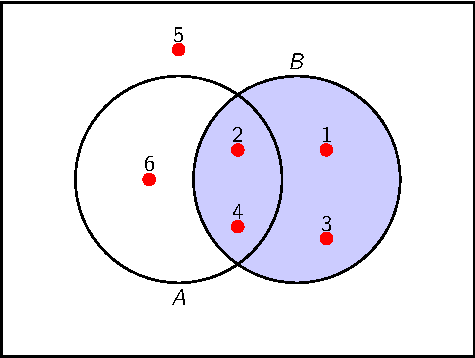
\includegraphics[width=0.4\linewidth]{figs/independencia-crop} \end{center}
\end{frame}

\setbeamercovered{transparent}
\begin{frame}
\frametitle{Exemplo}

\textbf{Pela definição intuitiva}:

\(P(A) = 1/2\),
\quad \(P(A|B) = P(A\cap B)/P(B) = \frac{2/6}{4/6} = 1/2\).

\(P(B) = 2/3\),
\quad \(P(B|A) = P(B\cap A)/P(A) = \frac{2/6}{3/6} = 2/3\).

Portanto: \(P(A|B) = P(A)\) e \(P(B|A) = P(B)\).

\textbf{Pela definição formal:}

\(P(A \cap B) = P(A)P(B) = \frac{1}{2} \cdot \frac{2}{3} = 1/3.\)

\(P(A \cap B) = \frac{2}{6} = 1/3\), assim \(P(A \cap B) = P(A)P(B).\)

Portanto, os eventos \(A\) e \(B\) são independentes. Saber que \(A\)
ocorreu não muda a probabilidade de \(B\) ocorrer e vice-versa.
\end{frame}

\setbeamercovered{transparent}
\begin{frame}
\frametitle{Exemplo 2.5 (livro)}

Suponha que um fabricante de sorvetes recebe \(20\%\) de todo o leite
que utiliza de uma fazenda \(F_1\), \(30\%\) de uma outra fazenda
\(F_2\) e \(50\%\) de \(F_3\).

Um órgão de fiscalização inspecionou as fazendas de surpresa e observou
que \(20\%\) do leite produzido por \(F_1\) estava adulterado por adição
de água, enquanto que para \(F_2\) e \(F_3\), essa proporção era de
\(5\%\) e \(2\%\), respectivamente.

Na indústria de sorvetes os galões de leite são armazenados em um
refrigerador sem identificação das fazendas. Para um galão escolhido ao
acaso, qual a probabilidade do leite estar adulterado?
\end{frame}


\setbeamercovered{transparent}
\begin{frame}
\frametitle{Partição do espaço amostral}

Dizemos que os eventos \(C_1, C_2, ..., C_k\) formam uma
\textbf{partição} do espaço amostral, se eles não tem interseção entre
si, e se sua união é igual ao espaço amostral. Isto é,

\[
C_i \cap C_j = \emptyset \quad \text{para} \quad i \not= j \quad
\text{e} \quad \bigcup_{i=1}^k C_i = \Omega.
\]

\begin{center}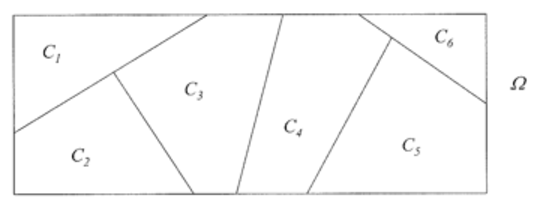
\includegraphics[width=0.6\linewidth]{figs/particao} \end{center}
\end{frame}

\setbeamercovered{transparent}
\begin{frame}
\frametitle{Exemplo 2.5 (livro)}

Seja \(A\) o evento ``o leite está adulterado'', podemos defini-lo
conforme a figura abaixo.


\begin{center}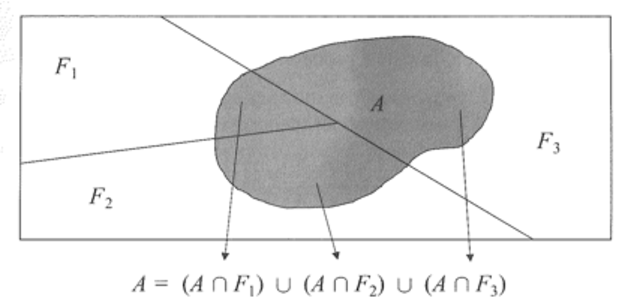
\includegraphics[width=0.6\linewidth]{figs/bayes} \end{center}


\end{frame}

\setbeamercovered{transparent}
\begin{frame}
\frametitle{Teorema de Bayes}

Podemos estar interessados também na probabilidade de uma amostra
adulterada ter sido obtida a partir da fazenda \(F_1\), ou seja,
\(P(F_1|A)\).
\begin{alertblock}{Teorema de Bayes}

Suponha que os eventos \(C_1, C_2, \ldots, C_k\) formem uma partição de
\(\Omega\) e que suas probabilidades sejam conhecidas. Suponha, ainda,
que para um evento \(A\), se conheçam as probabilidades \(P(A | C_i)\)
para todo \(i = 1, 2, \ldots, k.\) Então, para qualquer \(j\),

\[
P(C_j | A ) = \frac{P(C_j)P(A | C_j)}{\sum_{i=1}^k P(C_i)P(A | C_i)},
\quad j = 1,2, \ldots,k.
\]
\end{alertblock}
\end{frame}

\setbeamercovered{transparent}
\begin{frame}
\frametitle{Exemplo 2.6 (livro)}

Usando o exemplo anterior, podemos agora calcular a probabilidade de que
o leite adulterado tenha sido obtido a partir da fazenda \(F_1\).

\begin{align*}
P(F_1|A) &= \frac{P(F_1)P(A|F_1)}
{P(F_1)P(A|F_1) + P(F_2)P(A|F_2) + P(F_2)P(A|F_2)} \\
  &= \frac{0,2 \times 0,2}
{0,2 \times 0,2 + 0,3 \times 0,05 + 0,5 \times 0,02} \\
  &= 0,615.
\end{align*}

De maneira similar, podemos obter \(P(F_2|A)\) e \(P(F_3|A)\).
\end{frame}

\setbeamercovered{transparent}
\begin{frame}
\frametitle{Exercícios recomendados}

\begin{itemize}
\item
  Seção \(2.1\) Ex. \(1, 2, 3, 4\) e \(5\).
\item
  Seção \(2.2\) Ex. \(1, 2, 3, 4, 5, 6\).
\end{itemize}
\end{frame}

\end{document}